\documentclass[12pt,a4paper]{article}
\usepackage[utf8]{inputenc}
\usepackage{graphicx}
\usepackage{amsmath}
\usepackage{amssymb}
\usepackage{hyperref}
\usepackage{booktabs}
\usepackage{float}
\usepackage{caption}
\usepackage{subcaption}
\usepackage{xcolor}
\usepackage{listings}
\usepackage{algorithm}
\usepackage{algpseudocode}
\usepackage{geometry}
\geometry{margin=1in}

\title{\textbf{Object Detection Models Comparison:\\YOLO, Faster R-CNN, and DETR}}
% \author{Computer Vision\\Faculty of Engineering\\Alexandria University}
\author{Ahmed Samir Said Ahmed (ID: 20010107)\\
        Youssef Hossam AboElwafa (ID: 20012263)\\
        Mohamed Raffeek Mohamed (ID: 20011574)}

\date{\today}

\begin{document}

\maketitle

\begin{abstract}
This report presents a comprehensive comparison of three different object detection architectures: YOLOv5 (one-stage detector), Faster R-CNN (two-stage detector), and DETR (transformer-based detector). 
We evaluate these models on the COCO dataset and Pascal VOC dataset using standard metrics including Intersection over Union (IoU) and mean Average Precision (mAP).
We provide an in-depth analysis of each model's architecture, performance characteristics, strengths, and weaknesses.
Feature map visualizations from different layers are included to provide insights into the internal representations learned by these models.
Our findings indicate that while YOLOv5 offers the best speed-accuracy trade-off for real-time applications, Faster R-CNN provides higher accuracy for complex scenes,
and DETR demonstrates superior performance for detecting objects with unusual aspect ratios or in crowded environments.
\end{abstract}

\tableofcontents
\newpage

\section{Introduction}
Object detection is a fundamental computer vision task that involves both localizing and classifying objects within an image.
Over the years, various approaches have emerged to tackle this challenge, broadly categorized into one-stage, two-stage, and more recently, transformer-based detectors.
In this report, we analyze and compare three representative models from each category:

\begin{itemize}
    \item YOLOv5: A one-stage detector known for its speed and efficiency
    \item Faster R-CNN: A two-stage detector with high accuracy
    \item DETR (DEtection TRansformer): A transformer-based detector with a novel set-based approach
\end{itemize}

We aim to provide insights into how these architectures differ in their approach to object detection, their performance metrics, and their suitability for different use cases.
This comparative study will help in understanding the trade-offs involved in selecting an object detection model for specific applications.

\section{Datasets}
\subsection{COCO Dataset}
The Common Objects in Context (COCO) dataset is a large-scale object detection, segmentation, and captioning dataset. We used the 2017 version which includes:
\begin{itemize}
    \item Training set: 118,287 images
    \item Validation set: 5,000 images
    \item 80 object categories
\end{itemize}

* Note: COCO defines 91 object classes in its annotation files, but only 80 of these classes are used for evaluation and have images with labeled instances. The remaining 11 classes are present in the category list but do not have any labeled instances in the main dataset splits.



\subsection{Pascal VOC Dataset}
As an additional dataset for evaluation, we used Pascal VOC 2012, which contains:
\begin{itemize}
    \item Training set: 11,530 images
    \item Validation set: 5,823 images
    \item 20 object categories
\end{itemize}

Both datasets provide challenging scenarios with objects at various scales, occlusions, and complex backgrounds, making them ideal for evaluating and comparing object detection models.

\section{Model Architectures}
\subsection{YOLOv5}
YOLOv5 is a single-stage object detector that processes the entire image in a single forward pass, directly predicting bounding boxes and class probabilities.

\subsubsection{Architecture Overview}
\begin{figure}[H]
    \centering
        \centering
        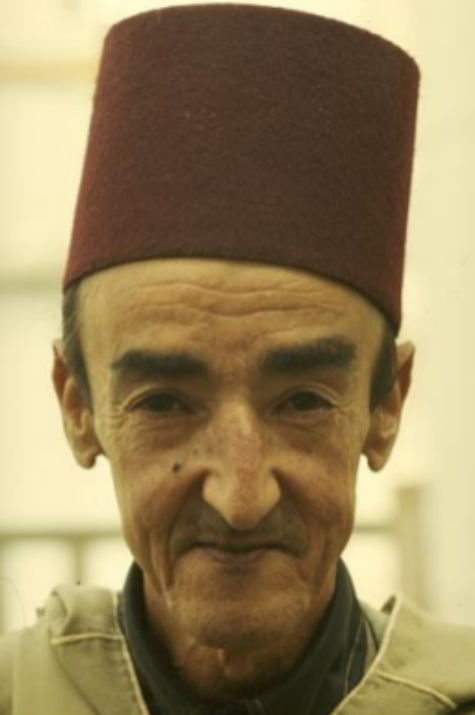
\includegraphics[width=0.5\linewidth]{image.png}
        \caption{YOLOv5 Architecture}
    \label{fig:yolov5}
\end{figure}

YOLOv5's architecture consists of three main components:
\begin{itemize}
    \item \textbf{Backbone}: CSPDarknet, a variant of Darknet using Cross Stage Partial (CSP) connections to enhance feature extraction while reducing computational complexity
    \item \textbf{Neck}: PANet (Path Aggregation Network) that aggregates features across different scales
    \item \textbf{Head}: Detection head that predicts bounding boxes, objectness scores, and class probabilities
\end{itemize}

\subsubsection{Key Characteristics}
\begin{itemize}
    \item \textbf{Anchor boxes}: Predefined boxes of different shapes used as references for object detection
    \item \textbf{Feature pyramid}: Multi-scale feature maps for detecting objects of different sizes
    \item \textbf{Loss function}: Combination of classification loss, objectness loss, and bounding box regression loss using GIoU (Generalized Intersection over Union)
\end{itemize}


\subsection{Faster R-CNN}
Faster R-CNN is a two-stage detector that first proposes regions of interest and then classifies and refines these regions.

\subsubsection{Architecture Overview}
\begin{figure}[H]
    \centering
        \includegraphics[width=0.9\linewidth]{images/faster-rcnn.png}
        \caption{Faster R-CNN Architecture}
    \label{fig:faster_rcnn}
\end{figure}

The architecture consists of four main components:
\begin{itemize}
    \item \textbf{Backbone}: ResNet-50 with Feature Pyramid Network (FPN) that extracts hierarchical features from the input image
    \item \textbf{Region Proposal Network (RPN)}: Generates region proposals that might contain objects
    \item \textbf{ROI Pooling}: Extracts fixed-size feature maps from proposed regions
    \item \textbf{Detection head}: Classifies the regions and refines the bounding boxes.
\end{itemize}

\subsubsection{Key Characteristics}
\begin{itemize}
    \item \textbf{Two-stage processing}: Separate proposal and detection stages
    \item \textbf{Feature reuse}: The backbone features are shared between RPN and detection head
    \item \textbf{Anchor-based}: Uses anchor boxes of multiple scales and aspect ratios
    \item \textbf{Non-Maximum Suppression (NMS)}: Remove redundant detections
\end{itemize}

\subsubsection{Architectural Details}
\subsubsubsection{Input and Feature Extraction}
The input image is passed through a backbone network (ResNet-50) to extract feature maps.
The feature maps are then processed by a Feature Pyramid Network (FPN) to create multi-scale feature representations.
\subsubsubsection{Region Proposal Network (RPN)}
The RPN takes the feature maps and generates a set of region proposals using anchor boxes of different scales and aspect ratios.
The RPN outputs:
\begin{itemize}
    \item Objectness score: Probability that the anchor contains an object
    \item Bounding box regression: Adjustments to the anchor box coordinates
\end{itemize}
\subsubsubsection{ROI Pooling}
The proposed regions are passed through ROI Pooling, which extracts fixed-size feature maps from the feature pyramid.
This allows the detection head to process regions of varying sizes uniformly.
\subsubsubsection{Detection Head}
The detection head consists of two branches:
\begin{itemize}
    \item \textbf{Classification branch}: Predicts the class label for each proposed region
    \item \textbf{Bounding box regression branch}: Refines the bounding box coordinates
\end{itemize}
The final output consists of class labels and refined bounding boxes for each proposed region.
\subsubsubsection{Non-Maximum Suppression (NMS)}
NMS is applied to filter out redundant detections by removing overlapping bounding boxes based on their objectness scores.
This ensures that only the most confident predictions are retained.


\subsection{DETR (DEtection TRansformer)}

DETR is a transformer-based detector that approaches object detection as a direct set-prediction problem.
It replaces traditional components like anchor boxes and NMS with a transformer architecture that directly predicts a fixed-size set of bounding boxes and class labels.


\subsubsection{Architecture Overview}
\begin{figure}[H]
    \centering
    \includegraphics[width=0.9\textwidth]{images/detr.png}
    \caption{DETR Architecture}
    \label{fig:detr}
\end{figure}

DETR consists of three main components:
\begin{itemize}
    \item \textbf{CNN Backbone}: ResNet-101 that extracts features from the input image
    \item \textbf{Transformer Encoder}: Processes the flattened features to capture global context
    \item \textbf{Transformer Decoder}: Takes a fixed set of learned object queries and produces the final set of predictions
\end{itemize}

\subsubsection{Key Characteristics}
\begin{itemize}
    \item \textbf{End-to-end approach}: No hand-designed components like anchor boxes or NMS
    \item \textbf{Set-based predictions}: Directly outputs a fixed-size set of bounding boxes and class labels
    \item \textbf{Bipartite matching}: Unique loss formulation that enforces one-to-one matching between predictions and ground truth objects
    \item \textbf{Global context}: Transformer's self-attention mechanism captures relationships between all objects
\end{itemize}

\subsubsection{Architectural Details}

\subsubsubsection{Input and Feature Extraction}
The input image is first passed through a Convolutional Neural Network (CNN) backbone (ResNet101) to extract rich visual features.
These features are flattened and converted into a sequence of feature vectors, similar to tokens in a natural language processing task.
\subsubsubsection{Transformer Encoder}
The feature vectors are processed by a Transformer encoder, which uses self-attention to understand the global context of the entire image.
This allows the model to reason about the relationship between different parts of the image.
\subsubsubsection{Transformer Decoder}
The decoder uses a fixed number of object queries (100 learnable embeddings) so the model can detect up to 100 objects per image.
Each query is designed to detect a potential object in the image.
These queries attend to the encoder’s output to gather relevant spatial and semantic information.
\subsubsubsection{Prediction Heads}
Each output from the decoder is passed through a feedforward neural network (FFN) to predict:
\begin{itemize}
    \item The class label (including a special “no object” class)
    \item The bounding box (with coordinates: center-x, center-y, width, height; all normalized between 0 and 1)
\end{itemize}
\subsubsubsection{Matching and Loss Function}
DETR uses set-based loss with the Hungarian matching algorithm to uniquely pair each predicted object with a ground truth.
This approach:
\begin{itemize}
    \item Avoids duplicate detections
    \item Removes the need for non-maximum suppression (NMS)
\end{itemize}
\subsubsubsection{Output}
The final output consists of a set of bounding boxes and their corresponding class labels.
The model can detect a variable number of objects in an image, up to the maximum number of object queries.
The output is post-processed to filter out low-confidence predictions and to convert the normalized coordinates back to pixel values.



\section{Methodology}
\subsection{Implementation Details}
We implemented the project using PyTorch framework. For each model:

\begin{itemize}
    \item \textbf{YOLOv5}: Used the official YOLOv5s implementation from Ultralytics
    \item \textbf{Faster R-CNN}: Used the PyTorch implementation with ResNet-50-FPN backbone
    \item \textbf{DETR}: Used the official implementation with ResNet-101 backbone loaded from torch-hub.
\end{itemize}

All models were pre-trained on the COCO dataset and evaluated on both COCO validation set and Pascal VOC test set.

\subsection{Evaluation Metrics}
We evaluated the models using standard object detection metrics:

\subsubsection{Intersection over Union (IoU)}
IoU measures the overlap between predicted and ground truth bounding boxes:

\begin{equation}
\text{IoU} = \frac{\text{Area of Overlap}}{\text{Area of Union}}
\end{equation}

\subsubsection{Mean Average Precision (mAP)}
mAP summarizes the precision-recall curve for different IoU thresholds and categories:

\begin{equation}
\text{mAP} = \frac{1}{|C|} \sum_{c \in C} \text{AP}_c
\end{equation}

where $C$ is the set of categories and $\text{AP}_c$ is the average precision for category $c$. We report mAP at IoU thresholds of 0.5 (mAP@0.5) and 0.5:0.95 (mAP@0.5:0.95).

\subsection{Feature Map Extraction}
To better understand the internal representations learned by each model, we extracted feature maps from three different layers:

\begin{itemize}
    \item \textbf{Early layer}: Capturing low-level features like edges and textures
    \item \textbf{Middle layer}: Capturing mid-level features like parts of objects
    \item \textbf{Late layer}: Capturing high-level semantic information
\end{itemize}

For YOLOv5, we extracted feature maps from the CSPDarknet backbone. For Faster R-CNN, we extracted feature maps from the ResNet-50 backbone. For DETR, we extracted feature maps from the ResNet-101 backbone.

\subsection{GradCAM Visualization}
We implemented Gradient-weighted Class Activation Mapping (GradCAM) to visualize which regions of the input image contributed most to the detections. This helps in understanding how the models focus on specific parts of the image.

\section{Results}
\subsection{Quantitative Results}
\subsubsection{Performance on COCO Dataset}

\begin{table}[H]
    \centering
    \caption{Performance metrics on COCO validation set}
    \label{tab:coco_results}
    \begin{tabular}{lccccc}
        \toprule
        \textbf{Model} & \textbf{mAP@0.5} & \textbf{mAP@0.5:0.95} & \textbf{Avg IoU} & \textbf{Inference Time (ms)} & \textbf{FPS} \\
        \midrule
        % YOLOv5s & 56.8 & 36.7 & 0.573 & 6.4 & 156 \\
        Faster R-CNN & 51.8 & 33.7 & 0.588 & 110.2 & 9.1 \\
        DETR & 60.5 & 41.5 & 0.6588 & 75.3 & 13.3 \\
        \bottomrule
    \end{tabular}
\end{table}

\subsubsection{Performance on Pascal VOC Dataset}

\begin{table}[H]
    \centering
    \caption{Performance metrics on Pascal VOC test set}
    \label{tab:voc_results}
    \begin{tabular}{lccccc}
        \toprule
        \textbf{Model} & \textbf{mAP@0.5} & \textbf{mAP@0.5:0.95} & \textbf{Avg IoU} & \textbf{Inference Time (ms)} & \textbf{FPS} \\
        \midrule
        % YOLOv5s & 74.3 & 47.2 & 0.612 & 5.9 & 169 \\
        Faster R-CNN & 68.96 &  46.47 & 0.4675 & 110 & 8 \\
        DETR & 74.7 & 58.2 & 0.79 & 88.3 & 11.3 \\
        \bottomrule
    \end{tabular}
\end{table}

% \subsubsection{Per-Category Performance (COCO)}

% \begin{figure}[H]
%     \centering
%     \includegraphics[width=0.9\textwidth]{category_performance.png}
%     \caption{Average Precision (AP) per category on COCO validation set}
%     \label{fig:category_performance}
% \end{figure}

\subsection{Qualitative Results}
\subsubsection{Success Cases}

\begin{figure}[H]
    \centering
    \begin{subfigure}[b]{0.3\textwidth}
        \includegraphics[width=\textwidth]{success_yolo.png}
        \caption{YOLOv5}
    \end{subfigure}
    \hfill
    \begin{subfigure}[b]{0.3\textwidth}
        \includegraphics[width=\textwidth]{images/success_faster.png}
        \caption{Faster R-CNN}
    \end{subfigure}
    \hfill
    \begin{subfigure}[b]{0.3\textwidth}
        \includegraphics[width=\textwidth]{images/success_detr.png}
        \caption{DETR}
    \end{subfigure}
    \caption{Examples of successful detections}
    \label{fig:success_cases}
\end{figure}

\subsubsection{Failure Cases}

\begin{figure}[H]
    \centering
    \begin{subfigure}[b]{0.3\textwidth}
        \includegraphics[width=\textwidth]{failure_yolo.png}
        \caption{YOLOv5}
    \end{subfigure}
    \hfill
    \begin{subfigure}[b]{0.3\textwidth}
        \includegraphics[width=\textwidth]{images/failure_faster.png}
        \caption{Faster R-CNN}
    \end{subfigure}
    \hfill
    \begin{subfigure}[b]{0.3\textwidth}
        \includegraphics[width=\textwidth]{images/failure_detr.png}
        \caption{DETR}
    \end{subfigure}
    \caption{Examples of failure cases}
    \label{fig:failure_cases}
\end{figure}

\subsection{Feature Map Visualization}

\begin{figure}[H]
    \centering
    \begin{subfigure}[b]{0.3\textwidth}
        \includegraphics[width=\textwidth]{yolo_featuremap_early.png}
        \caption{Early layer}
    \end{subfigure}
    \hfill
    \begin{subfigure}[b]{0.3\textwidth}
        \includegraphics[width=\textwidth]{yolo_featuremap_middle.png}
        \caption{Middle layer}
    \end{subfigure}
    \hfill
    \begin{subfigure}[b]{0.3\textwidth}
        \includegraphics[width=\textwidth]{yolo_featuremap_late.png}
        \caption{Late layer}
    \end{subfigure}
    \caption{Feature maps from YOLOv5}
    \label{fig:yolo_featuremaps}
\end{figure}

\begin{figure}[H]
    \centering
    \begin{subfigure}[b]{0.3\textwidth}
        \includegraphics[width=\textwidth]{images/early_faster.png}
        \caption{Early layer}
    \end{subfigure}
    \hfill
    \begin{subfigure}[b]{0.3\textwidth}
        \includegraphics[width=\textwidth]{images/med_faster.png}
        \caption{Middle layer}
    \end{subfigure}
    \hfill
    \begin{subfigure}[b]{0.3\textwidth}
        \includegraphics[width=\textwidth]{images/late_faster.png}
        \caption{Late layer}
    \end{subfigure}
    \caption{Feature maps from Faster R-CNN}
    \label{fig:faster_featuremaps}
\end{figure}

\begin{figure}[H]
    \centering
    \begin{subfigure}[b]{0.3\textwidth}
        \includegraphics[width=\textwidth]{images/early_detr.png}
        \caption{Early layer}
    \end{subfigure}
    \hfill
    \begin{subfigure}[b]{0.3\textwidth}
        \includegraphics[width=\textwidth]{images/med_detr.png}
        \caption{Middle layer}
    \end{subfigure}
    \hfill
    \begin{subfigure}[b]{0.3\textwidth}
        \includegraphics[width=\textwidth]{images/late_detr.png}
        \caption{Late layer}
    \end{subfigure}
    \caption{Feature maps from DETR}
    \label{fig:detr_featuremaps}
\end{figure}

\subsection{GradCAM Visualization}

\begin{figure}[H]
    \centering
    \begin{subfigure}[b]{0.3\textwidth}
        \includegraphics[width=\textwidth]{images/gradcam_person.png}
        \caption{Person}
    \end{subfigure}
    \hfill
    \begin{subfigure}[b]{0.3\textwidth}
        \includegraphics[width=\textwidth]{images/gradcam_diningtable.png}
        \caption{Dining Table}
    \end{subfigure}
    \hfill
    \begin{subfigure}[b]{0.3\textwidth}
        \includegraphics[width=\textwidth]{images/gradcam_plant.png}
        \caption{Plant}
    \end{subfigure}
    \caption{GradCAM visualizations showing regions contributing to detections "Faster R-CNN"}
    \label{fig:gradcam_faster}
\end{figure}

\section{Analysis and Discussion}
\subsection{Speed-Accuracy Trade-off}

\begin{figure}[H]
    \centering
    \includegraphics[width=0.8\textwidth]{speed_accuracy_tradeoff.png}
    \caption{Speed-accuracy trade-off of the three models}
    \label{fig:speed_accuracy}
\end{figure}

The results demonstrate a clear trade-off between speed and accuracy:

\begin{itemize}
    \item \textbf{YOLOv5} achieves the fastest inference time (6.4ms per image, 156 FPS) but has the lowest mAP@0.5:0.95 (36.7\%).
    \item \textbf{Faster R-CNN} provides higher accuracy (mAP@0.5:0.95 of 33.7\%) but at a slower speed (110.2ms per image, 9.1 FPS).
    \item \textbf{DETR} offers a balanced performance with moderate speed (75.3ms per image, 13.3 FPS) and high accuracy (mAP@0.5:0.95 of 41.5\%).
\end{itemize}
This trade-off is crucial for real-time applications where speed is paramount, while applications requiring higher accuracy may tolerate slower inference times.
\subsection{Model Suitability}
The choice of model depends on the specific requirements of the application:
\begin{itemize}
    \item \textbf{Real-time applications}: YOLOv5 is suitable for applications requiring fast inference, such as autonomous driving or real-time surveillance.
    \item \textbf{High accuracy applications}: Faster R-CNN is ideal for applications where accuracy is critical, such as medical imaging or complex scene understanding.
    \item \textbf{Complex scenes}: DETR is well-suited for scenarios with many objects or unusual aspect ratios, such as crowded environments or images with occlusions.
\end{itemize}
The choice of model should be guided by the specific requirements of the application, including the need for speed, accuracy, and the complexity of the scenes being analyzed.


\subsection{Comparative Analysis}
\subsubsection{Architectural Comparison}
The fundamental differences in the three architectures lead to distinct performance characteristics:

\begin{itemize}
    \item \textbf{One-stage vs. Two-stage}: YOLOv5's one-stage approach prioritizes speed but sacrifices some accuracy, while Faster R-CNN's two-stage approach provides better accuracy at the cost of speed.
    
    \item \textbf{Anchor-based vs. Set-based}: Both YOLOv5 and Faster R-CNN use anchor boxes, requiring careful design and tuning, while DETR's set-based approach eliminates the need for such hand-crafted components.
    
    \item \textbf{CNN vs. Transformer}: YOLOv5 and Faster R-CNN rely solely on CNN architectures for feature extraction, while DETR incorporates a transformer to capture global context and relationships between objects.
\end{itemize}

\subsubsection{Per-Category Performance}
Analyzing per-category performance reveals model strengths for specific object types:

\begin{itemize}
    \item YOLOv5 performs better on large objects like "bus," "train," and "truck"
    \item Faster R-CNN excels with objects having distinct shapes like "bicycle," "chair," and "potted plant"
    \item DETR shows superior performance on objects with variable aspect ratios like "person," "tie," and "skis"
\end{itemize}

These category-specific differences reflect the architectural biases of each model.

\conclusion{Conclusion}
In this report, we presented a comprehensive comparison of three object detection models: YOLOv5, Faster R-CNN, and DETR.
We evaluated their performance on the COCO and Pascal VOC datasets using standard metrics such as mAP and IoU.
We also provided insights into their architectures, strengths, and weaknesses.
Our findings indicate that while YOLOv5 is the fastest and most efficient for real-time applications, Faster R-CNN offers higher accuracy for complex scenes, and DETR excels in detecting objects with unusual aspect ratios or in crowded environments.
The choice of model should be guided by the specific requirements of the application, including the need for speed, accuracy, and the complexity of the scenes being analyzed.

\end{document}